\chapter{Stellar Structure and Evolution}
\label{stellarstruc}
The field of stellar structure and evolution is wide and it is possible to study numerous aspects of it. In this section, a brief introduction to the theory of stellar structure and evolution is given. This is based on mainly \citet{christensen2008lecture} and \citet{kippenhahn1990stellar}.   

It is difficult to paint a general picture of a "star". There are numerous types of stars, varying in observable properties such as magnitude and effective temperature, but also indirect properties such as their inner structures. Assumptions and simplifications are therefore necessary in order to  give a comprehensible  representation of a star. First, and foremost, a star is always assumed to be in \textit{hydrostatic equilibrium}, meaning that physics on a macroscopic level adapts to the surroundings on a timescale much faster than the \textit{free-fall time} (i.e. the time it takes until the interstellar cloud has contracted to a single point. The star is also assumed to have none or little rotation such that it can be treated as spherically symmetric. Magnetic fields are commonly assumed to not be present in the star. These assumption are of course very crude, as we know that stars do indeed rotate and have magnetic fields. However, the assumptions provides us the possibility to give a rough estimate on the conditions in a star. 

A star in hydrostatic equilibrium balances its own gravitation with the gas pressure. By looking at an infinitesimal small mass element $dm$ at a distance $r$ from the center, one can derive

\begin{equation}
    \frac{dP}{dr} = - \frac{GM(r)}{r^2}\rho
\end{equation}

\noindent where $G$ is the gravitational constant and $P$ is the pressure. This equation states that the pressure obtained from gas and radiation must be equal to that of gravitation in order to maintain hydrostatic equilibrium. A star is also assumed to follow the equation of mass-conservation 
\begin{equation}
    \frac{dM(r)}{dr}  = 4\pi r^2 \rho,
\end{equation}

\noindent where $M(r)$ is the mass of a spherical shell of  radius $r$. Combining the two equations yields

\begin{equation}
    -\frac{dP}{dM(r)} = \frac{G}{4\pi}\frac{M(r)}{r^4}.
    \end{equation}

\noindent From these equations it is possible to derive expressions for the minimum value of the central pressure $P_c$, the mean pressure $\Tilde{P}$ and temperature $\Tilde{T}$ for the case of a homogeneous star. Here, no knowledge on the composition is required, only the mass distribution.

The energy in a star is defined by the energy creation (and loss)  in a certain layer. The conservation is then defined

\begin{equation}
     \frac{dL}{dM(r)} = \eta = \eta_{nuc} - \eta_{\nu} - T\frac{\partial s}{\partial T},
\end{equation} 

\noindent where $\eta_{nuc}$ is nuclear energy generation rate, $\eta_{\nu}$ is the neutrino loss rate and $T\frac{\partial s}{\partial T}$ is the gravitational energy rate describing energy that is released or absorbed by the contraction or expansion of the star. The energy can be transported through radiation. The temperature gradient required to carry the entire luminosity of a star by radiation can be written as 

\begin{equation}
	\frac{dT}{dr} = -\frac{3 \rho}{64\pi^2 \sigma }\frac{\kappa L}{r^4 T^3},
\end{equation}

\noindent where L is the luminosity, $\kappa$ is the opacity, $\rho$ is the density and $\sigma$ is the Stefan-Boltzmann constant. This equation is valid as long a the \textit{diffusion approximation} is valid. This breaks down at the stellar surface. In this case the full, and much more complicated, equations of radiative transfer must be solved.

For a more thorough description of stellar structure, the properties of the matter need to be assessed. Describing the thermodynamical properties in detail is no simple task, but the fundamental assumption is that at any point in the star, the gas is assumed to be in \textit{thermodynamic equilibrium}, which means that there are no net macroscopic flows. This approximation ensures that instead of considering detailed reactions between particles, the average properties of the gas can be described by local state variables. The relations between these specifies the \textit{equation of state} (EOS) of the gas. It is also assumed that there is no change in the gas conditions over the distance of the mean-free-path of a particle located in the gas, or over the time between collisions. These assumptions are well applied in stellar interiors, but in order to describe conditions in the atmosphere, a more detailed description is needed. 

Since temperatures in the interiors are high, most of the gas will be fully ionized, and thereby have no internal degrees of freedom. Interactions b (collisions) between particles can be neglected, hence the gas is an approximate \textit{ideal gas} following the ideal-gas law

\begin{equation}
    PV = N k_B T,
\end{equation}

\noindent where $N$ is the number of particles in a gas with volume V, and $k_B$ is Boltzmann's constant. From this, general relations between pressure and internal energy can be derived. Stellar structure and evolution solves both equations of hydrostatic equilibrium and the EOS of the star. The modules used in this project will be described in \chapref{compute}. 


\section{Energy transport by convection}
\label{sec:energybyconvection}
When deriving the equations and variables for a star, it is usually assumed that the star can be treated as being spherically symmetric. In reality though, there will be fluctuations on small scales that has to be taken into account. The most considered of these instabilities or fluctuations is \textit{convection}. These can be treated as small perturbations. 

Convection can be described as macroscopic mass elements or "bubbles" that transports energy in a star. Elements that are hotter than their surroundings rises upwards carrying excess thermal energy. The displacement of the element grows exponentially and when the velocity becomes too large, nonlinear effects causes the thermal energy to be released into the surroundings. Thus, convection contributes by transporting energy, and mixing the gas elements. This has large consequences for the stellar evolution as we shall see in \secref{compute}. 

Whether a region in a star is stable against convection depends on whether the perturbation is allowed to grow under certain conditions. Therefore, it is a matter of \textit{convective instability}. Assuming that the mass elements do not exchange energy with the surroundings (during movement), and therefore moves adiabatically, it can be derived that 

\begin{equation}
\label{instability_eq}
    \nabla < \nabla_e + \frac{\phi}{\delta}\nabla_{\mu},
\end{equation}

\noindent describing the condition for convective stability. Here

\begin{equation}
    \nabla \equiv \left(\frac{d \ln T}{d \ln P}\right)_s, \qquad \nabla_e \equiv \left(\frac{\partial \ln T}{\partial \ln P}\right)_e, \qquad \nabla_\mu \equiv \left(\frac{\partial \ln \mu}{\partial \ln P}\right)_s.
\end{equation}

\noindent Here, the subscript $e$ means that the derivative is in relation to the element, whereas $s$ is the surrounding material. %Both $\nabla$ and $\nabla_\mu$, the derivatives are spatial with depth measured in P, whereas $\nabla_e$ varies T with the depth position of the element itself.
For the case where energy is transported by radiation or conduction only

\begin{equation}
    \nabla_{rad} \equiv \left(\frac{d \ln T}{d \ln P}\right)_{rad}, 
\end{equation}

\noindent temperature variation is described with depth. In a layer where all energy transport is either radiation or conduction, $\nabla = \nabla_{rad}$. Also, assuming that the element moves adiabatically such that 

\begin{equation}
\label{stability}
    \nabla_e = \nabla_{ad} \equiv \left(\frac{\partial \ln T}{\partial \ln P}\right)_{ad}
\end{equation}

\noindent and inserting in \eqref{instability_eq}, one arrives at

\begin{equation}
\label{stability2}
    \nabla_{rad} < \nabla_{ad} + \frac{\phi}{\delta} \nabla_\mu,
\end{equation}

known as the \textit{Ledoux criterion}. Under the assumptions mentioned earlier, this is the criteria for dynamical stability. It can be simplified further by assuming that the chemical composition is homogeneous such that $\mu$ is constant. This yields the \textit{Schwarzschild criterion} on the simple form:

\begin{equation}
\label{stability3}
    \nabla_{rad} < \nabla_{ad}.
\end{equation}

\noindent This assumption does not apply well to evolving stars where elements are not necessarily produced in  the same layer (as heavier elements are produced below lighter). 
Instability to convection thus occurs when the left hand side becomes larger than the right hand side. The small perturbations will grow until the layers is filled with convection. This occurs if

\begin{itemize}
    \item $L(r)/m(r)$, (the energy generation rate per unit mass within radius $r$) is large. In massive stars, this rate is an increasing function of temperature, thus increasing $L/m$ towards the center. Therefore these stars have convective cores.
    \item $\rho/T$ is large. Since $\rho/T^3$ increases rapidly in the photosphere, this usually occurs in cooler stars. 
    \item The opacity $\kappa$ is large. Stars with low surface temperatures usually have higher $\kappa$ in the outer layers. 
    \item $\nabla_{ad}$ is small. This happens in ionization zones.
\end{itemize}

To sum up, the first condition consequently allows for convection in the core of massive stars. The remaining conditions for outer layers of cooler stars. The different possibilities for the structures are illustrated on \figref{convectionzones}. 

\begin{figure}[htbp]
    \centering
    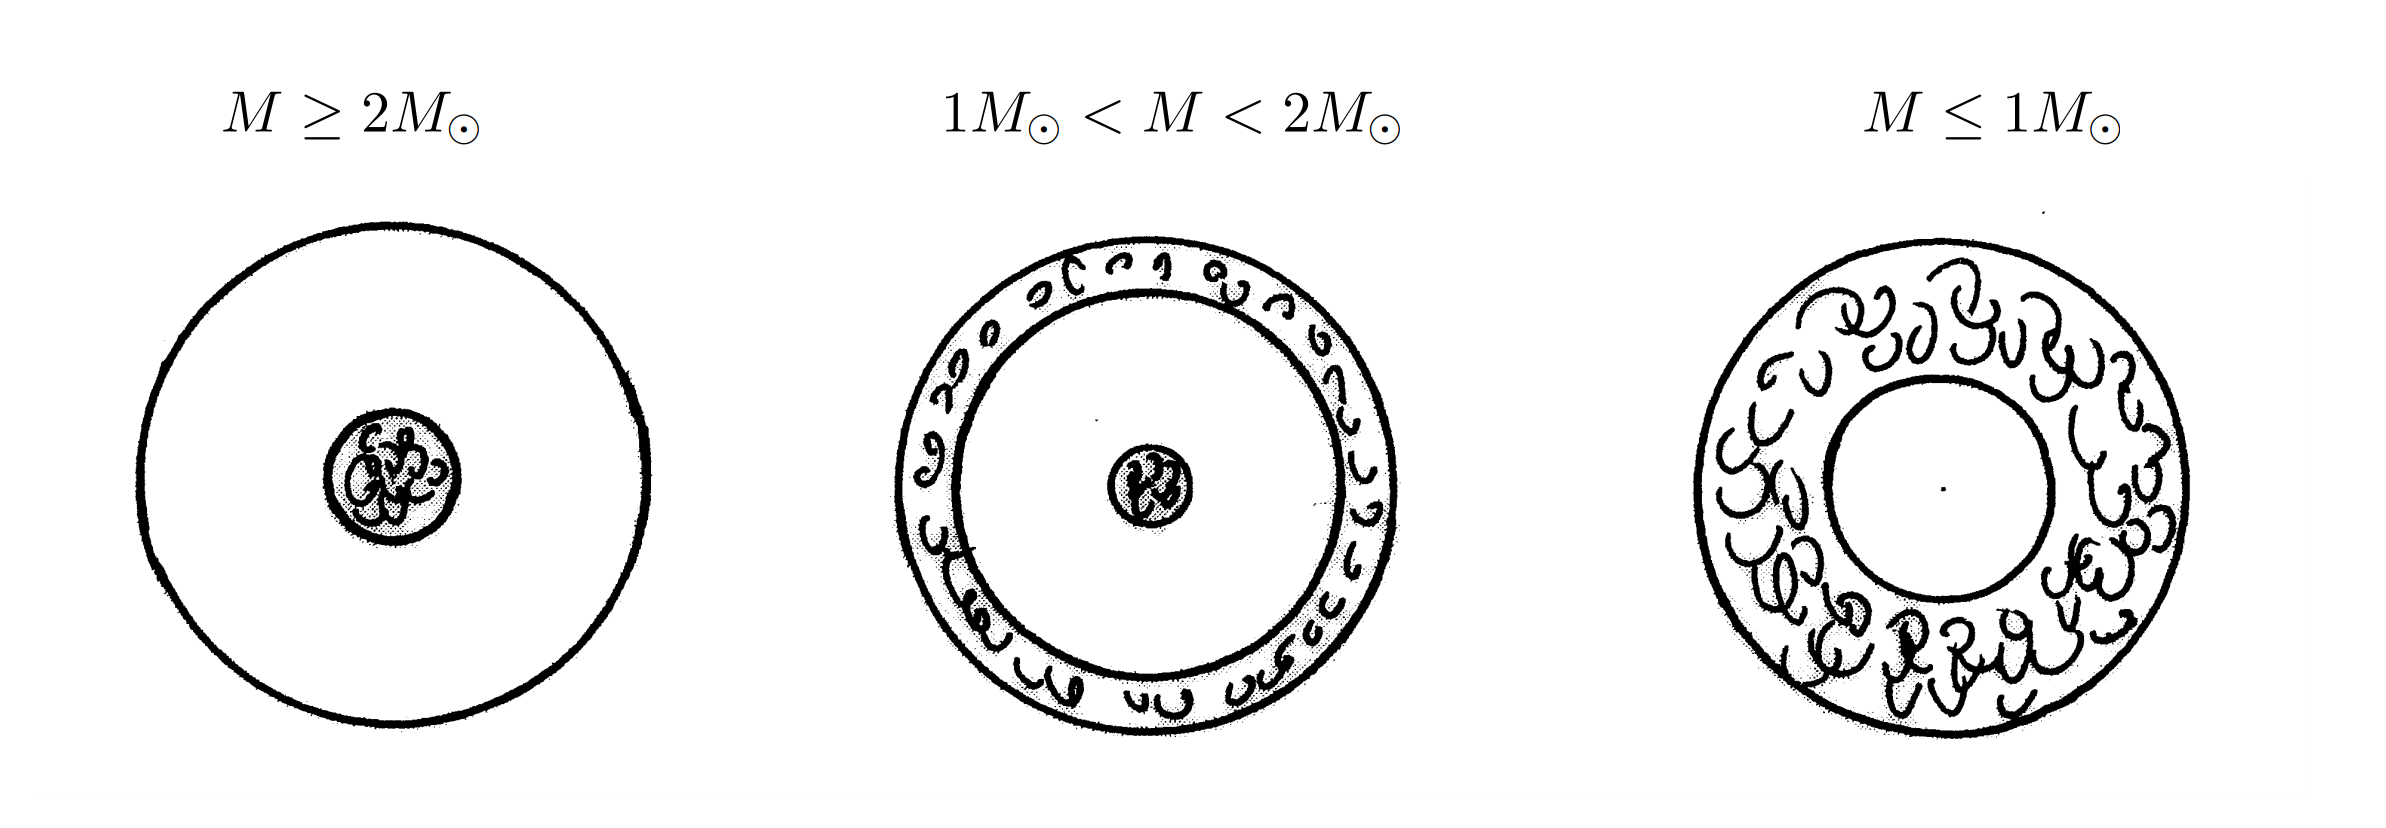
\includegraphics[width=1\textwidth]{convection_zones.png}
    \caption{Estimated occurrence of convection zones in main-sequence stars with different masses. Stars with masses higher than ~2 \msun have fully convective cores and only a very thin convective shell. Less massive stars with masses below 1\msun have deep convective envelopes. The stars in between marks the transition between the two. They have convective cores and a thin convective outer layer.}
    \label{convectionzones}
\end{figure}

The stars in this project lies in the \textit{intermediate mass} range which is usually stars of masses between 1.5\msun and 2.2\msun. They cover the transition from deep convective envelopes and convective cores. The motivation for using such stars will be discussed further in \secref{sec:why}.

If \eqref{stability2} leads to stability it follows that $\nabla = \nabla_{rad}$ for the entire layer. The  last possibility is that one of \eqref{stability2} and \eqref{stability3} says stability whereas the other says instability. This is called the Twilight zone, see \citep{kippenhahn1990stellar} for more details.
 
This prescription gives a very simplified picture of where convection is expected to occur within a star. However, in reality a local treatment is complicated since convective motion is not only dependent on local forces, but forces between layers as well (such as momentum and inertia). The border of a convective zone is thereby not well-defined and precise as elements accelerated from one layer might flow into another. This will be discussed further in \secref{sec:conv_prescriptions}. 
Convection flows in the laboratory is relatively well described by reasonable approximations. However, in stars convection is happening in much more violent conditions where compression of gas and turbulent motion depends on density, pressure and gravity of very high orders.  Taking such effects into consideration is not simple by any means, but efforts have been made to implement convection by making full two- and three-dimensional hydro dynamical simulations (e.g. \citet{nordlund19903}). Such codes do not treat the convection as separate homogeneous bubbles, but as a fully coupled time-dependent system. Such codes give a much more detailed and realistic picture of convection for single models. However, since the computation time for the full convective solution of a model is much longer than a simplified version, calculating a full track is not yet feasible. Therefore, the most used method is the \textit{standard mixing length theory} \citep{weiss2004cox}, which is a time-independent assessment. This is not sufficient to describe full hydrodynamical convection, but allows approximations to give a simplified local treatment, where convection can be described as macroscopic mass elements transferring energy. The mean free path is described with \textit{the mixing length}. There are several ways to implement this in stellar modeling which will be described in \secref{sec:conv_prescriptions}. 


\section[Stellar evolution through the HR-diagram]{Numerical results for stellar evolution through the HR-diagram}
This section describes the evolution of a star through numerically calculated stellar evolutionary tracks, mainly focusing on the main sequence (ms)) and immediate post-main sequence (pms) phases of intermediate mass stars

Stars are born from molecular clouds, collapsing under their own gravity. When the cloud reaches a the \textit{Jeans Mass}, the \textit{Jeans Criterion} is fulfilled, meaning that any perturbation will cause a free-fall collapse. This continues while the process happens isothermally until the free-fall time becomes similar to the timescale for thermal adjustment. The process then becomes adiabatic, stopping the rapid dynamical contraction and leaving behind a \textit{protostar} in hydrostatic equilibrium. Due to their low internal temperature and high opacity, these stars are fully convective. Thereby they are born on the \textit{Hayashi Track} where the contraction continues. This track is the beginning of the \textit{pre- main sequence phase}. As the star contracts and descends on the Hayashi track, the surface temperature (or effective temperature) is essentially constant while the luminosity decreases. The star heats up from the inside out since gas escapes the outer layers more easily. As the center becomes hotter, the opacity decreases and the convection zone slowly recedes. The star then leaves the Hayashi track and proceeds a radiative contraction on \textit{the Henyey track}. This causes the decreasing luminosity trend to reverse and the star becomes more luminous. Eventually the core temperatures will be sufficiently high to trigger the proton-proton reaction, converting H into deuterium ($^{2}\text{H}$) and thereafter $^3\text{He}$.\footnote{The full proton-proton chain is not yet completed since the temperature is still too low to burn hydrogen in full equilibrium.} 

%!!!Something happens here, understand it (Aearts p. 35)

As a result, a convective core is created. This will however disappear if the mass of the star is below 1.1\msun, whereas stars of higher mass will burn hydrogen in the cores through the \textit{CNO-cycle}. Accretion of mass continues on the pre-ms phase on a thermal timescale. Stars of masses larger than 9\msun moves so quickly into the MS phase that they are unobservable on the pre ms due to the thick shell of accreting mass, while stars of masses between 1.6-9\msun end their accretion of mass on the pre-ms. When the star begins burning hydrogen in full hydrostatic equilibrium it is born onto the \textit{zero-age main-sequence} (ZAMS). Stars below 0.08\msun never reaches ZAMS because their internal central temperature never becomes high enough to fuse hydrogen to helium in equilibrium. Instead they become degenerate, and are known as \textit{brown dwarfs}. Although stellar pulsations in brown dwarfs were theoretically predicted by \citet{palla2005pulsating} these pulsations have not yet been detected \citep{aerts2010, cody2014pulsation}. 

The ZAMS is where the star begins the life on the main-sequence where it spends 90 \% of its life burning H to He. The computed solutions from this stage on can be seen on \figref{stages}. The main sequence corresponding to the hydrogen burning in the core is defined as the phase between point 1 and 2. For all stars, the luminosity increases during this phase. The reason for this is that the hydrogen is converted into helium which causes the mean molecular weight to increase, which can be seen from

\begin{equation}
\label{meanmol}
\mu \simeq \frac{4}{3+5\text{X}-\text{Z}},
\end{equation}

REWRITE NEXT PART

\noindent where X, Y and Z is the hydrogen, helium and metal fraction respectively. The pressure must then compensate for the increase in gravitational pressure from the overlaying layers. Since $\text{P} \propto \rho \text{T}$ the core will start contracting to increase $\rho$. As a result of this contraction, gravitational potential energy energy is released, which further causes an increase in T (from the Virial theorem). Since the radiative flux is proportional to $\text{T}^{3}$ the temperature will increase, causing the opacity to decrease since $\sigma \propto \text{T}^{-3.5}$. Thus, the photons can escape more easily, and the luminosity increases. 

It is more complicated to explain the change in global parameters such as the effective temperature and radius. The radius increases in general as the star evolves, but the rate of this expansion is mass dependent. For stars that have low masses (close to 1\msun ) expansion is slow and the increase in luminosity will lead to an increase in the effective temperature as well, while it is the opposite for stars with higher masses and higher expansion rates. They will expand faster than the effective temperature increases, and will therefore cool down. 

%When hydrogen is exhausted in the core (point 2 on \figref{iben}) the star is left with a core consisting of helium. At this point the temperature in the core is too low to initiate helium burning, and the core is near isothermal. However, it is surrounded by a region where temperature is still high enough to burn hydrogen. This is called a \textit{shell source}. This provides the core with additional helium, hence increasing the mass causing it to contract and increasing the temperature until  
When hydrogen abundances get sufficiently low in the core, the star reaches the \textit{terminal-age main-sequence} (TAMS). Here, the core now consists of helium.
For intermediate mass stars,a noticeable feature is the "hook" following the ms, also known as the \textit{Henyey Hook} (not to be confused with the Henyey track). This is clearly depicted on \figref{stages2} As these type of stars have convective cores, the energy production will decrease uniformly throughout the core. The star will attempt to compensate for this by increasing the central temperature and keep the energy production up, hence causing the core to contract. As a result of the contraction, gravitational potential energy is released, where half is converted to thermal energy, heating up the core and essentially shifting the evolution to higher effective temperatures. This phase is in the order of a few megayears, which is extremely fast evolution compared to the main sequence (in the order of $10^{10}$ yrs. Therefore, studying a star in this exact phase is very difficult since a star can only be verified to be in this phase through modelling, as observations in color-magnitude diagrams cannot resolve it. From now on we will refer to this phase as the \textit{post main-sequence contraction phase}. At this point most of the energy production still comes from nuclear reactions, and the gravitational contribution is small in comparison.  It is surrounded by a region where temperature is still high enough to burn hydrogen, and slowly establishes a \textit{shell source}. This will however not be dominant until all hydrogen is exhausted. When this happens at point 3 on \figref{stages}, the evolution is accelerated and the star is no longer in equilibrium. The contracting core will thus be accompanied by an expanding envelope, causing the effective temperature to decrease. This phase will be referred to as the \textit{post- main sequence expansion phase}. The outer convection zone deepens until is reaches the layers where nuclear fusion has occures (the core). This is marked as point 5 and is also called \textit{first dredge up}. 

\begin{figure}[htbp]
    \centering
    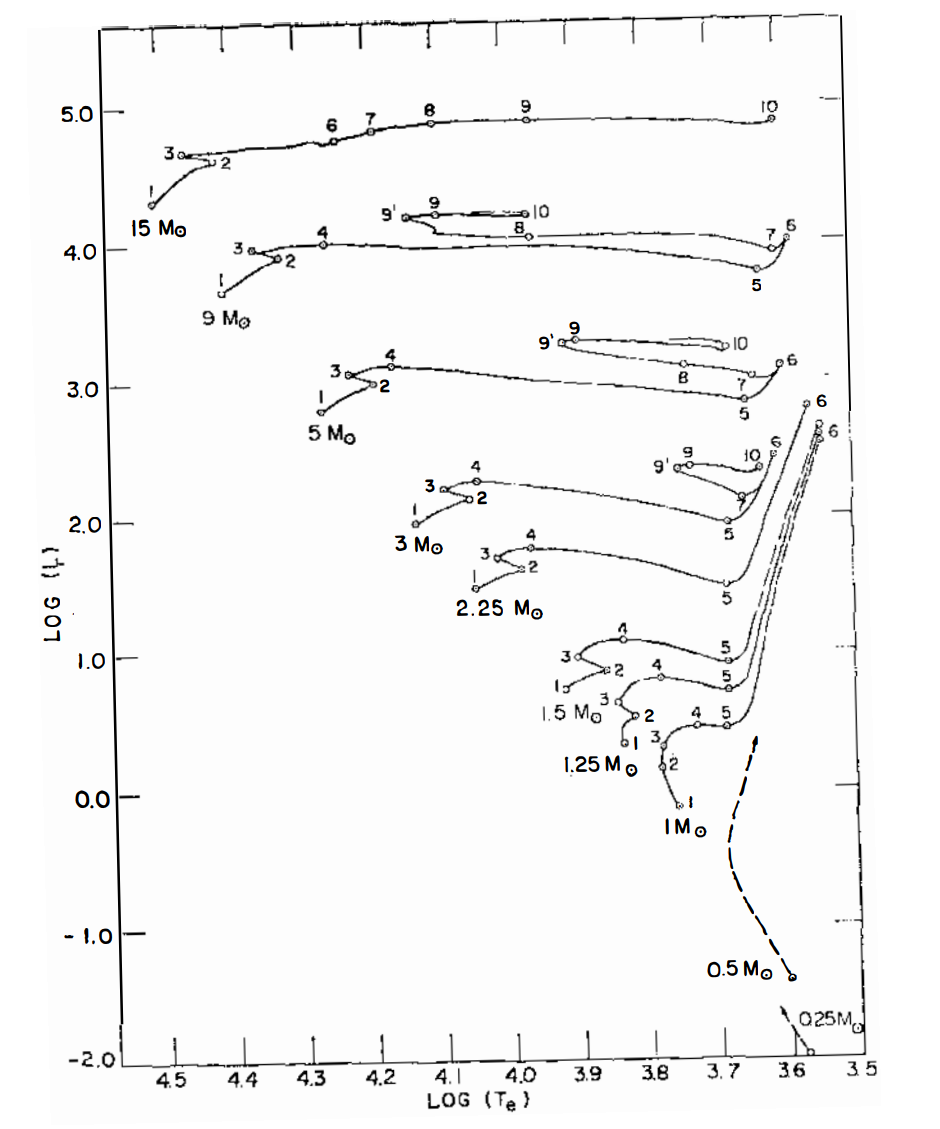
\includegraphics[width=0.8\textwidth]{iben.png}
    \caption{\citep{kippenhahn1990stellar} Stellar evolution tracks of masses ranging from 0.25\msun to 15\msun. The numbers indicate different stages in the evolution. Figure from \citet{iben1967stellar}.}
    \label{stages}
\end{figure}

\begin{figure}[htbp]
	\centering
	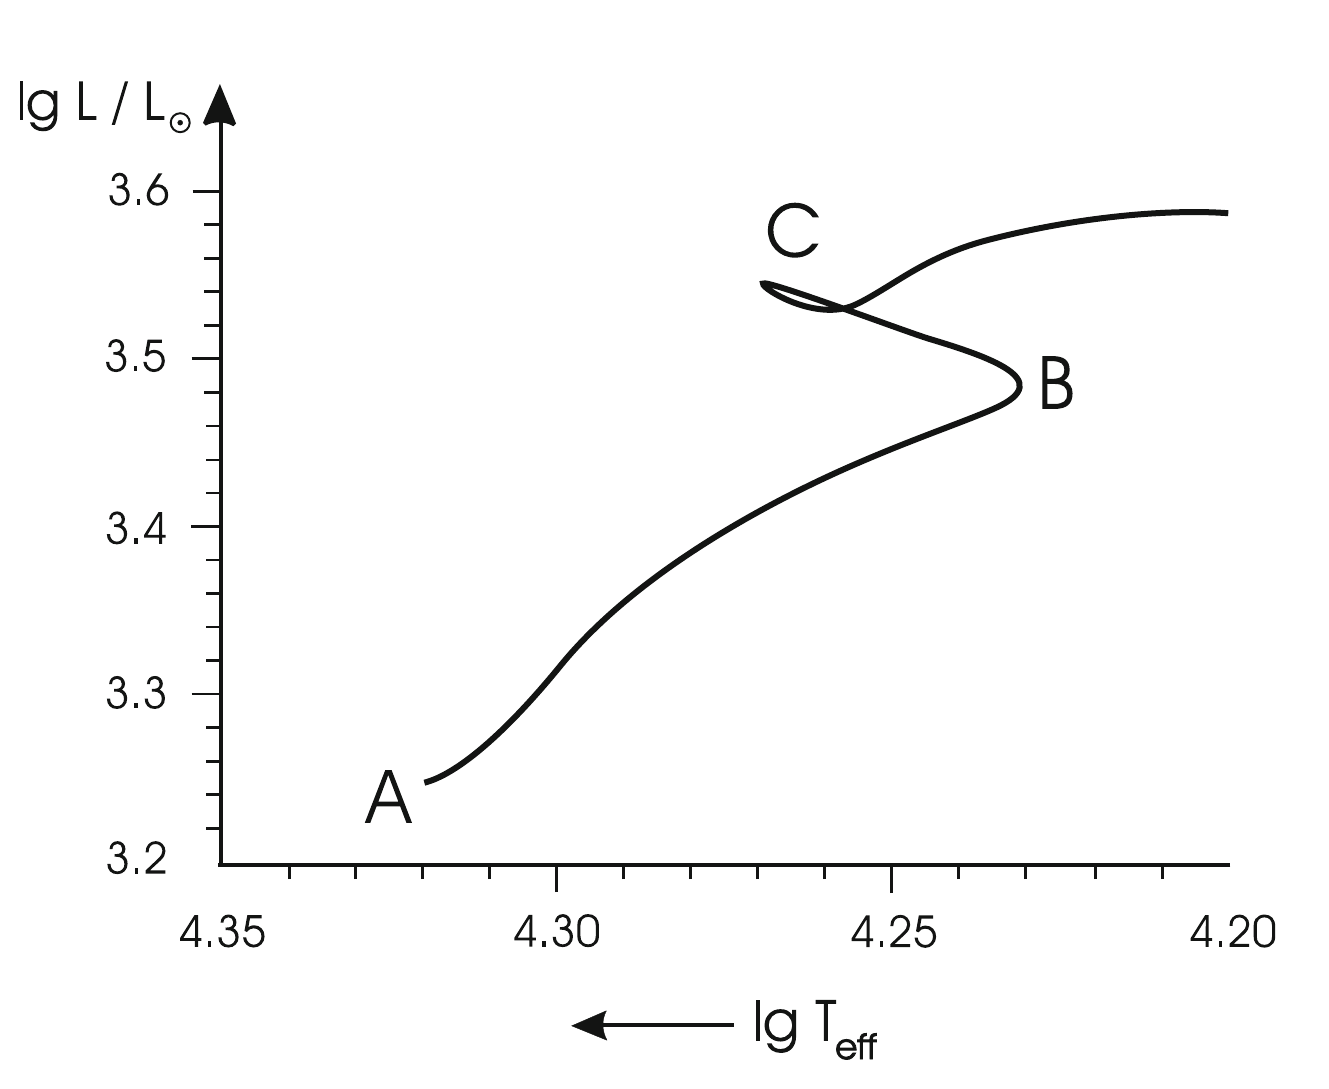
\includegraphics[width=0.8\textwidth]{STAGES.png}
	\caption{\citep{kippenhahn1990stellar} Stellar evolution track of a 5\msun star. The main sequence is marked between A and B, the post- ms contraction from B to C and the post -ms expansion is after C. Figure from \citep{kippenhahn1990stellar}.}
	\label{stages2}
\end{figure}

%As a consequence of this contraction, the conditions in the core become violent enough to ignite helium. 
At point 5-6 , the star will then move back up the Hyashi track as a red giant. The further evolution from then is largely depending on the mass. Stars with masses between 0.5<M<2.3\msun (relevant for this work) will have a degenerate helium core by the end of the main sequence (the exact cutoff depends on the initial metallicity in the star). The core contraction following the main-sequence continues until the reaches a temperature high enough to ignite helium in the core through the triple $\alpha$ process.   A thermal runaway known as \textit{helium-flash} occurs and lifts the degeneracy of the helium core, settling the star down on the \textit{horizontal branch} where it burns helium in the core and hydrogen in a shell (for stars with M<2.0\msun). 
 Stars with masses below 4-8\msun finish nuclear burning  at carbon or oxygen. By the end, their envelopes will be ejected into space through stellar winds, forming planetary nebulae. Left behind is the remnant, a white dwarf star.
  %The further evolution to this stage will not be discussed further in this work, but refer instead to \citet{kippenhahn1990stellar, christensen2008lecture} and \citet{weiss2004cox} for more details.   

Now we have seen how a star's luminosity changes as a function of effective temperature throughout its evolution. As mentioned in the beginning of the chapter, assumptions on hydrostatic equilibrium and equation of state can provide us with solutions that relates several other properties. The numerical solutions to the radius $R$,  surface gravity  $g$, core density $\rho$ and convective core mass are shown on \figref{stellarparams} as a function of time. The red lines indicate the beginning of the ms, post-ms contraction and post-ms expansion phases, respectively. As for the radius, the star contracts for the entirety of the pre-ms. As it burns hydrogen on the ms it slowly expands (as the temperature in the core decreases slightly with time) until the post-ms where it again contracts. After hydrogen exhaustion the star undergoes fast overall expansion. Another parameter which is highly relevant for the frequencies is the surface gravity, as we shall see in \secref{chap:asteroseismology}. From theory we know that $g \propto M/R^2$, which is equivalent to the numerical results shown on \figref{stellarparams}. The density in the center increases rapidly on the Hyashi track when the star contracts, and follows the linear tendency $\rho_c \propto \frac{3M}{\pi R^3}$ on the ms (by assuming $\rho$ is a linear function of the fractional radius $r$. At the immediate post-ms phase it increases again as the core contracts rapidly. 

An important parameter to also look at is the mass of the convective core. On the Hyashi track, the star is fully convective as it contracts. As the star burns hydrogen, the convective core mass slowly decreases until the point where .  On \figref{convcore}, numerical results for the convective core mass ratio to the total stellar mass is plotted as a function of stellar age in Gyrs for tracks with different masses. It can here be seen that higher stellar masses leads to higher convective core masses. Since stars with higher mass also have shorter lifetimes on the ms, which is also well-depicted on the figure as the convective core mass drops to zero when nuclear fusion in the core ends, which occurs sooner for higher masses. At this point, the core will not longer have high enough temperature to be convective. The smaller window on \figref{convcore} shows the convective core mass evolution on the pre-ms to the ms. Higher masses enter the hyashi track at a lower age than stars with smaller masses again indicating a faster evolution in general.  
%\begin{itemize}
 %   \item log g / age 
 %   \item log R / log g
 %   \item density / Radius
  %  \item log R / age
%    \item P / age
 %   \item P / R
%\end{itemize}

\begin{figure}[htbp]
    \centering
   \makebox[\textwidth][c]{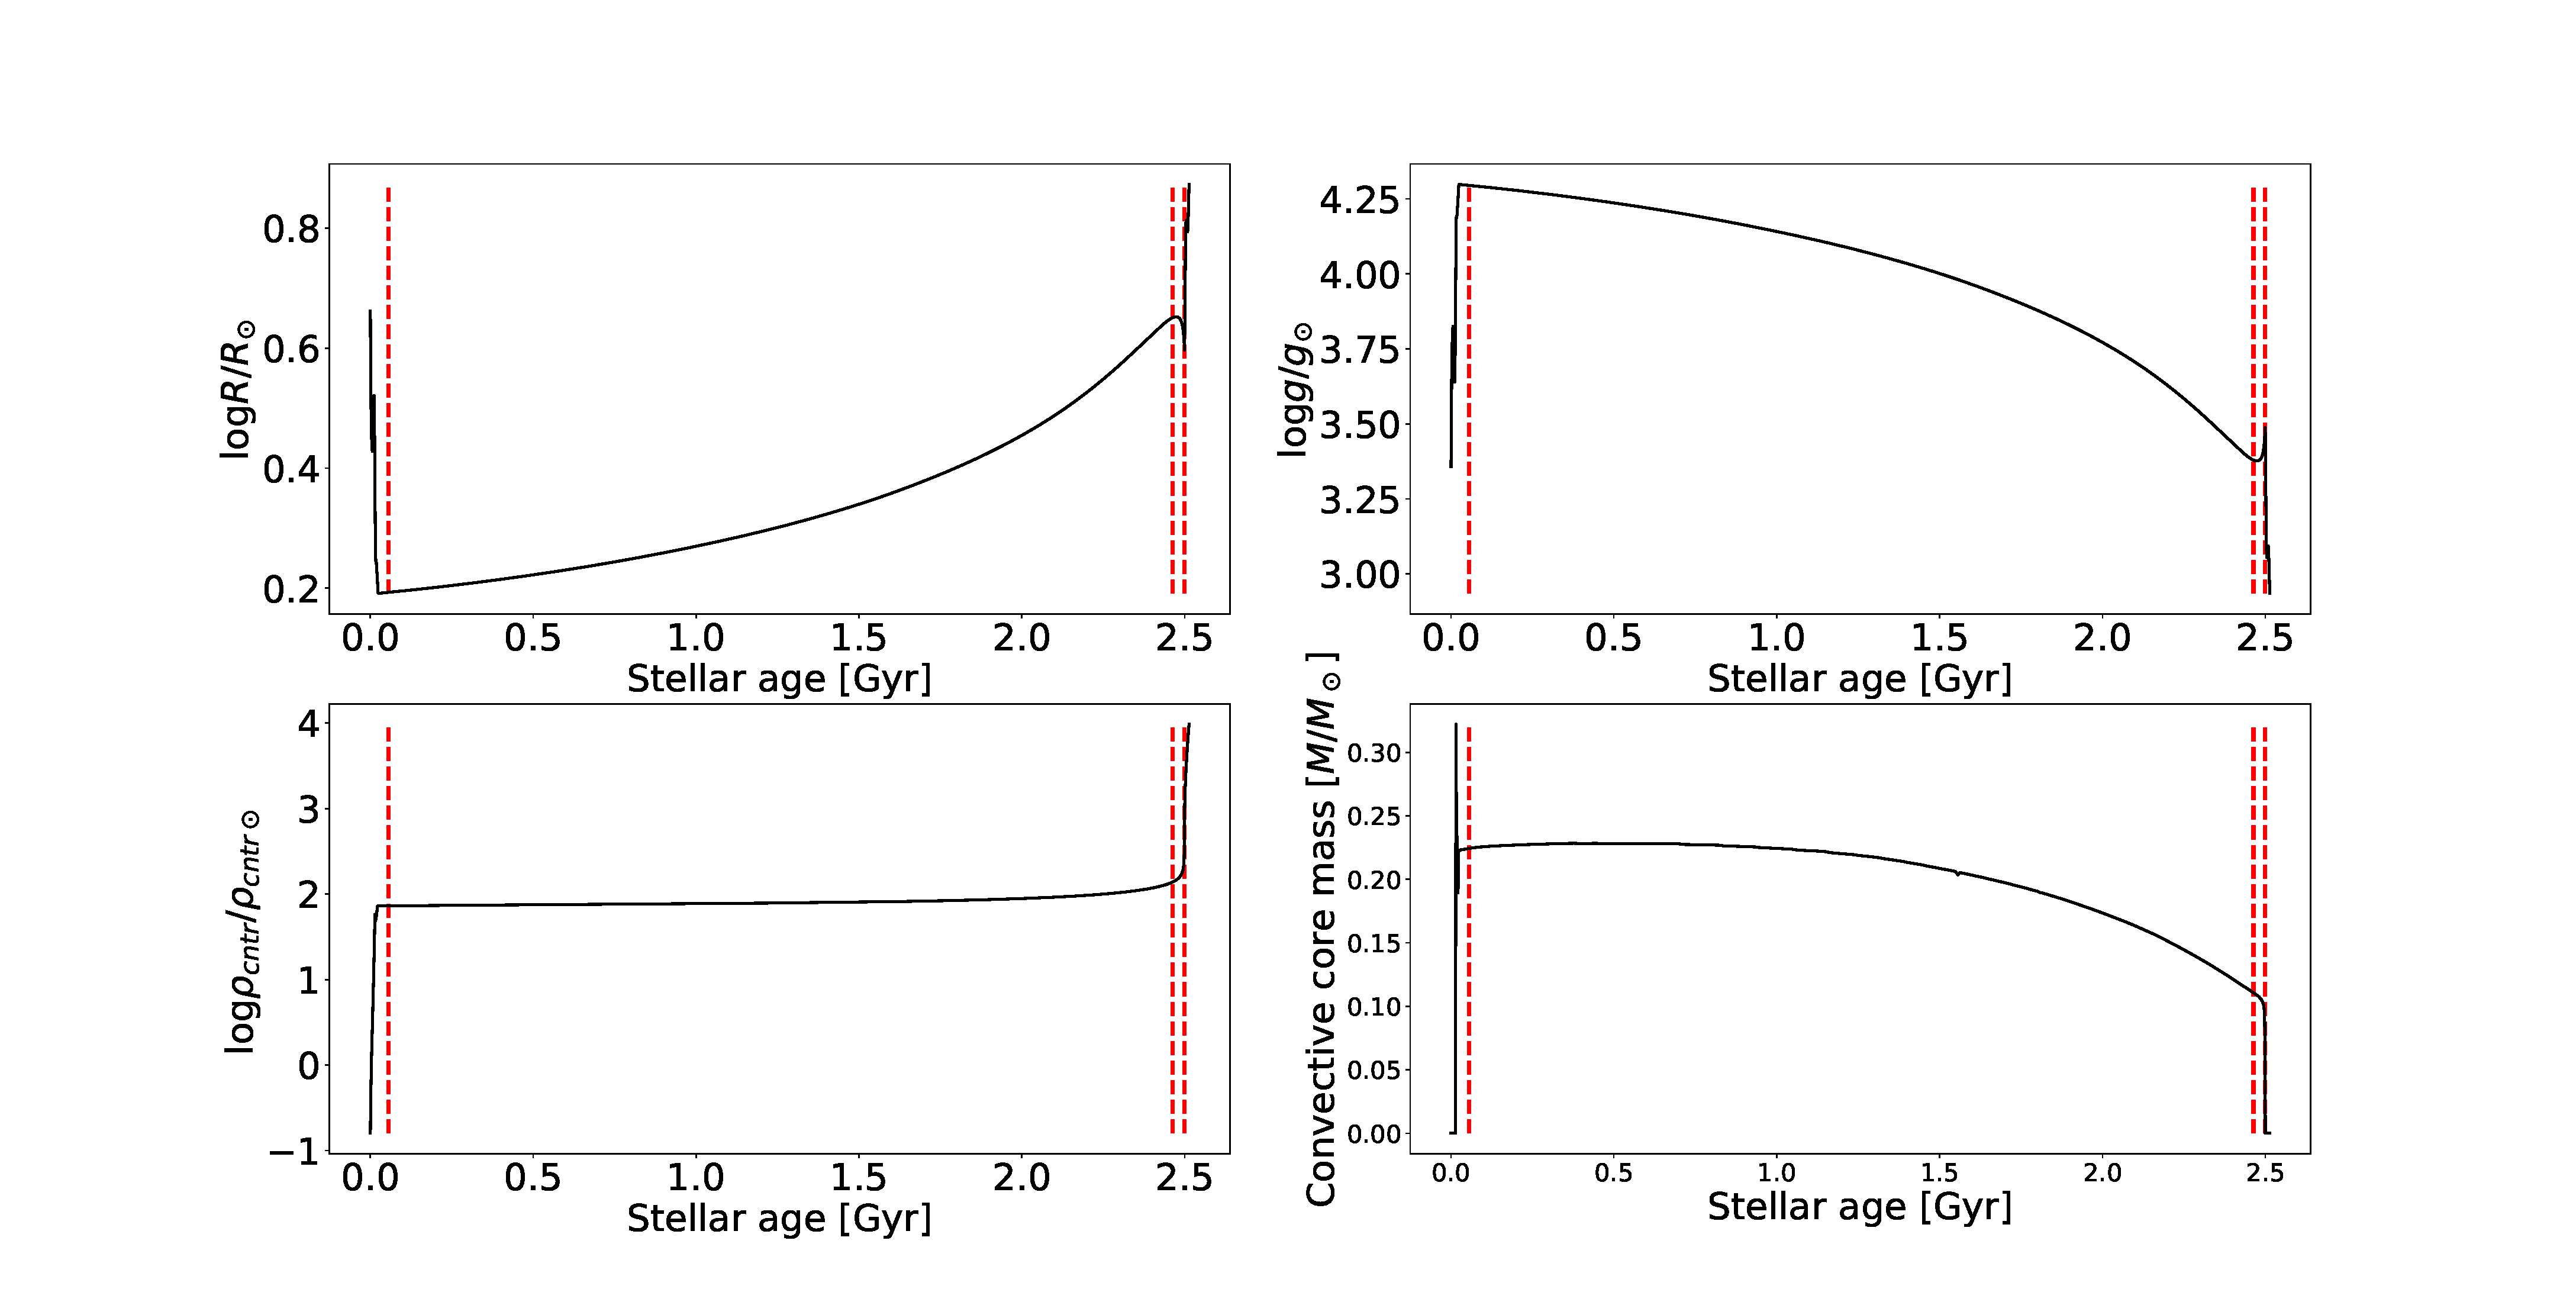
\includegraphics[width=1.4\textwidth]{stellar_params.eps}}%
    \caption{Numerically calculated stellar parameters for a track with 1.75\msun, X=0.65, Z=0.02, $\alpha_{mlt}$=0.5, $\alpha_{ov}$=0.3. The dashed lines marks the different stages of the evolution, leftmost being thew beginning of the main-sequence, middle one the post- main sequence contraction phase and rightmost the post-main sequence expansion phase.}
    \label{stellarparams}
\end{figure}


\begin{figure}[htbp]
    \centering
    \makebox[\textwidth][c]{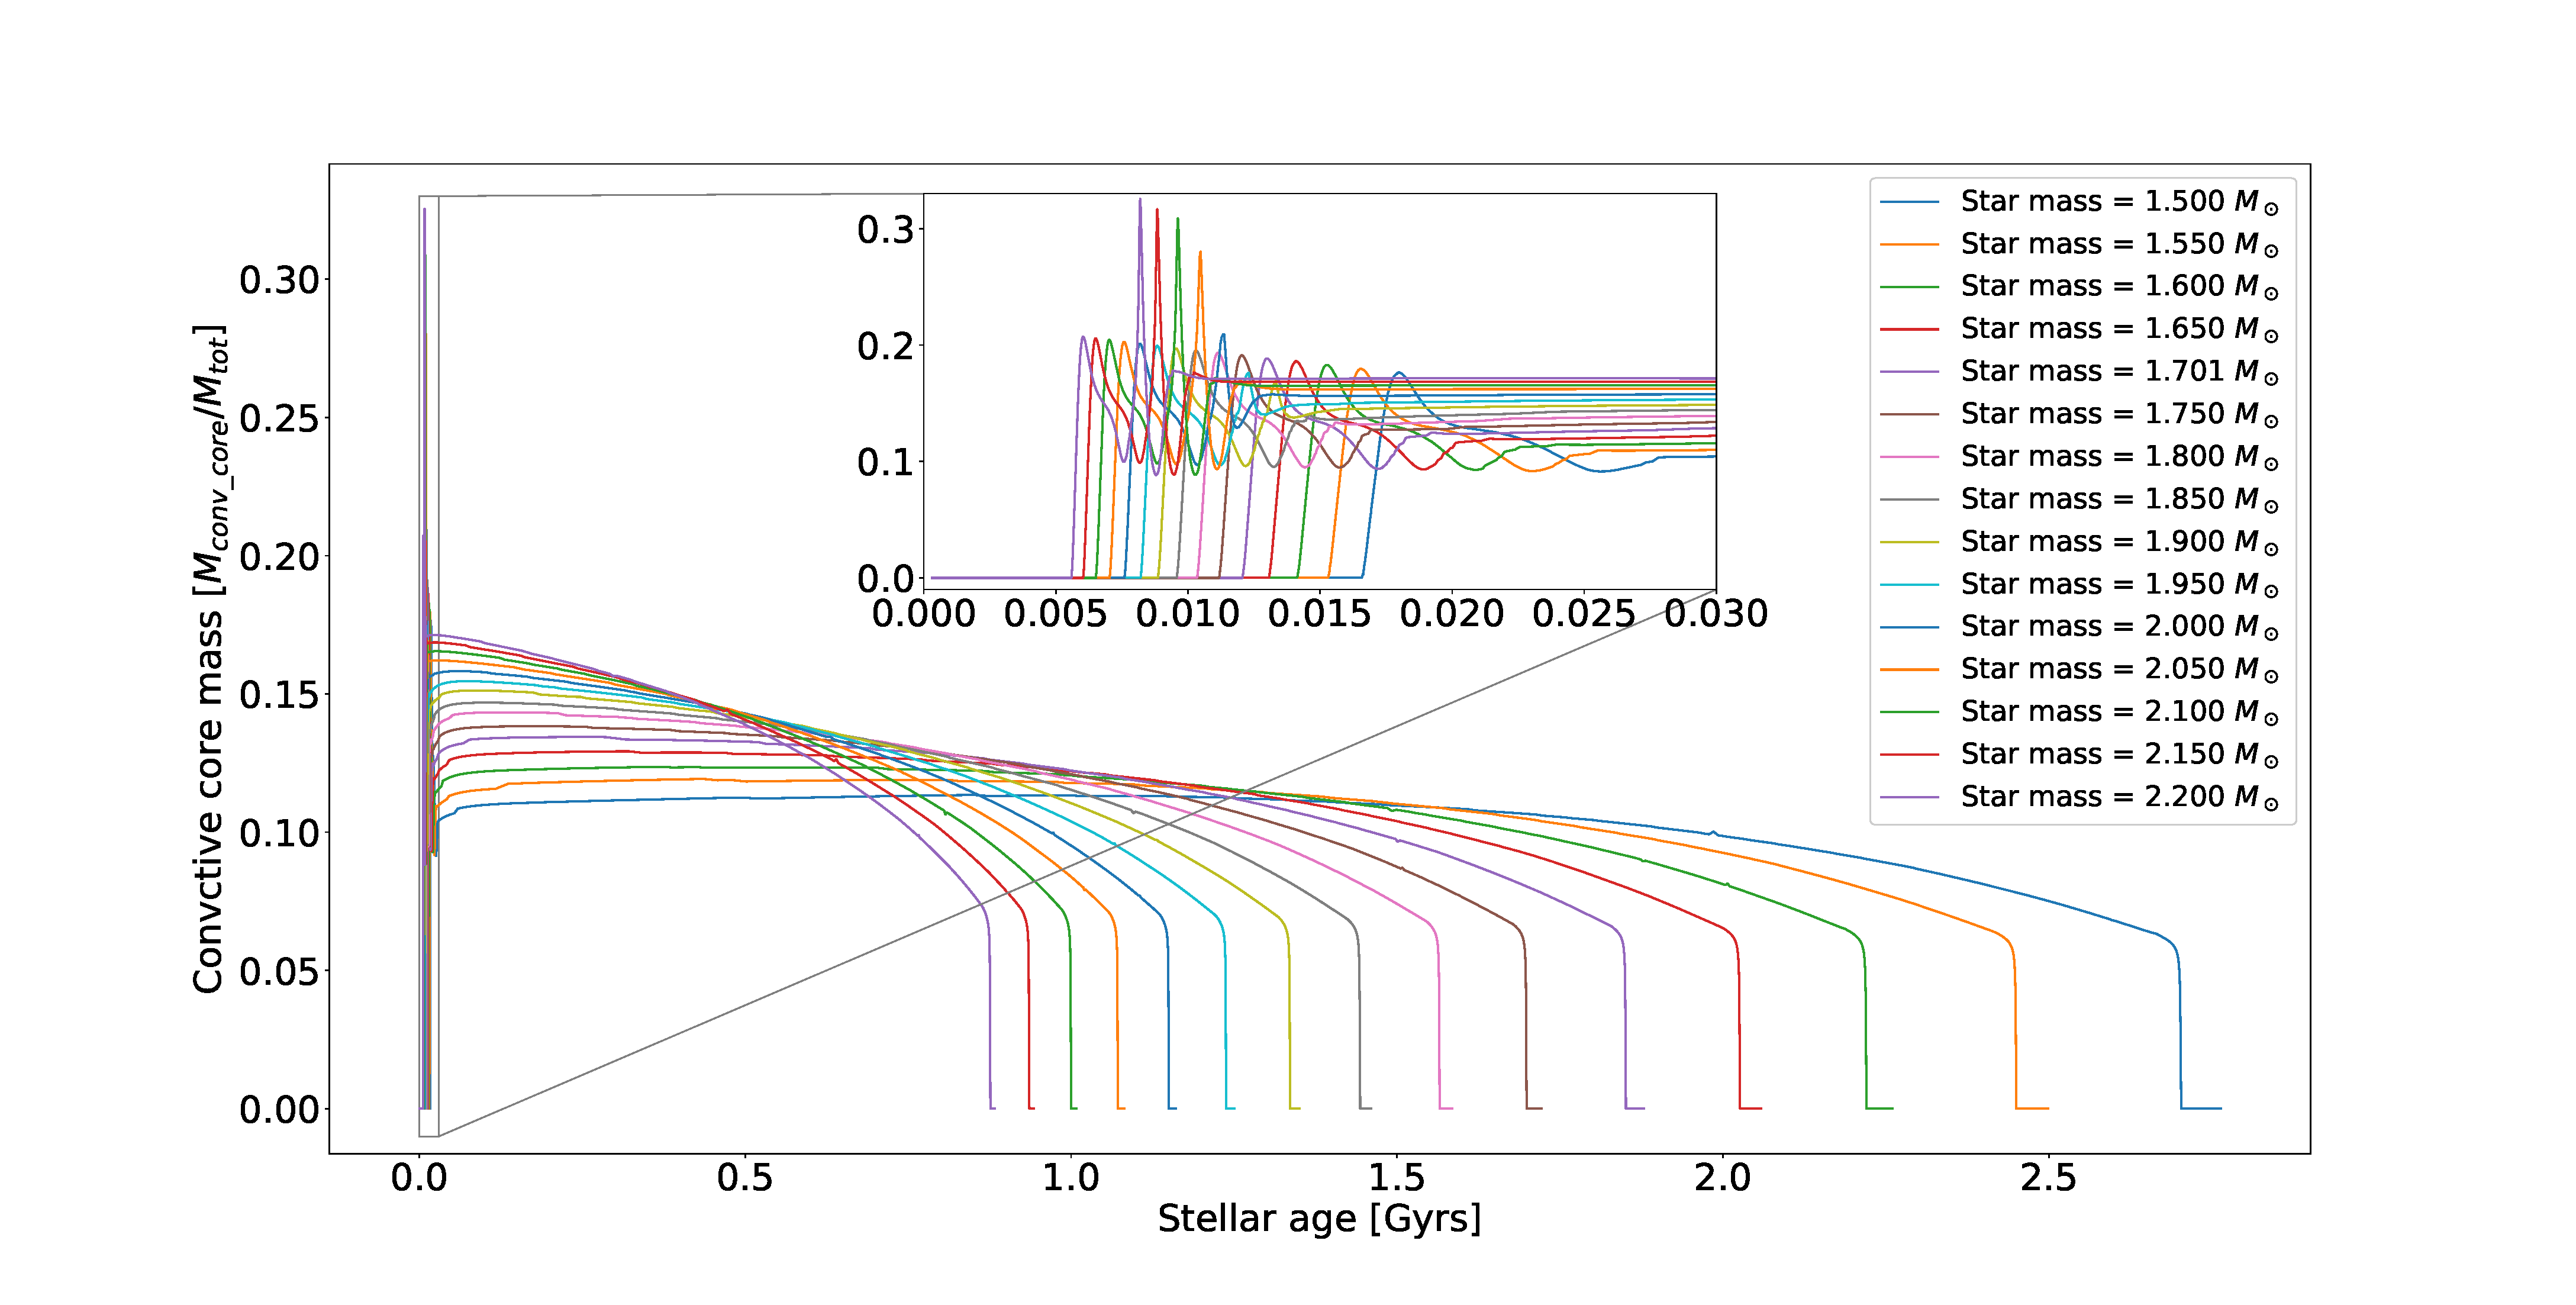
\includegraphics[width=1.4\textwidth]{conv_cores.eps}}%
    %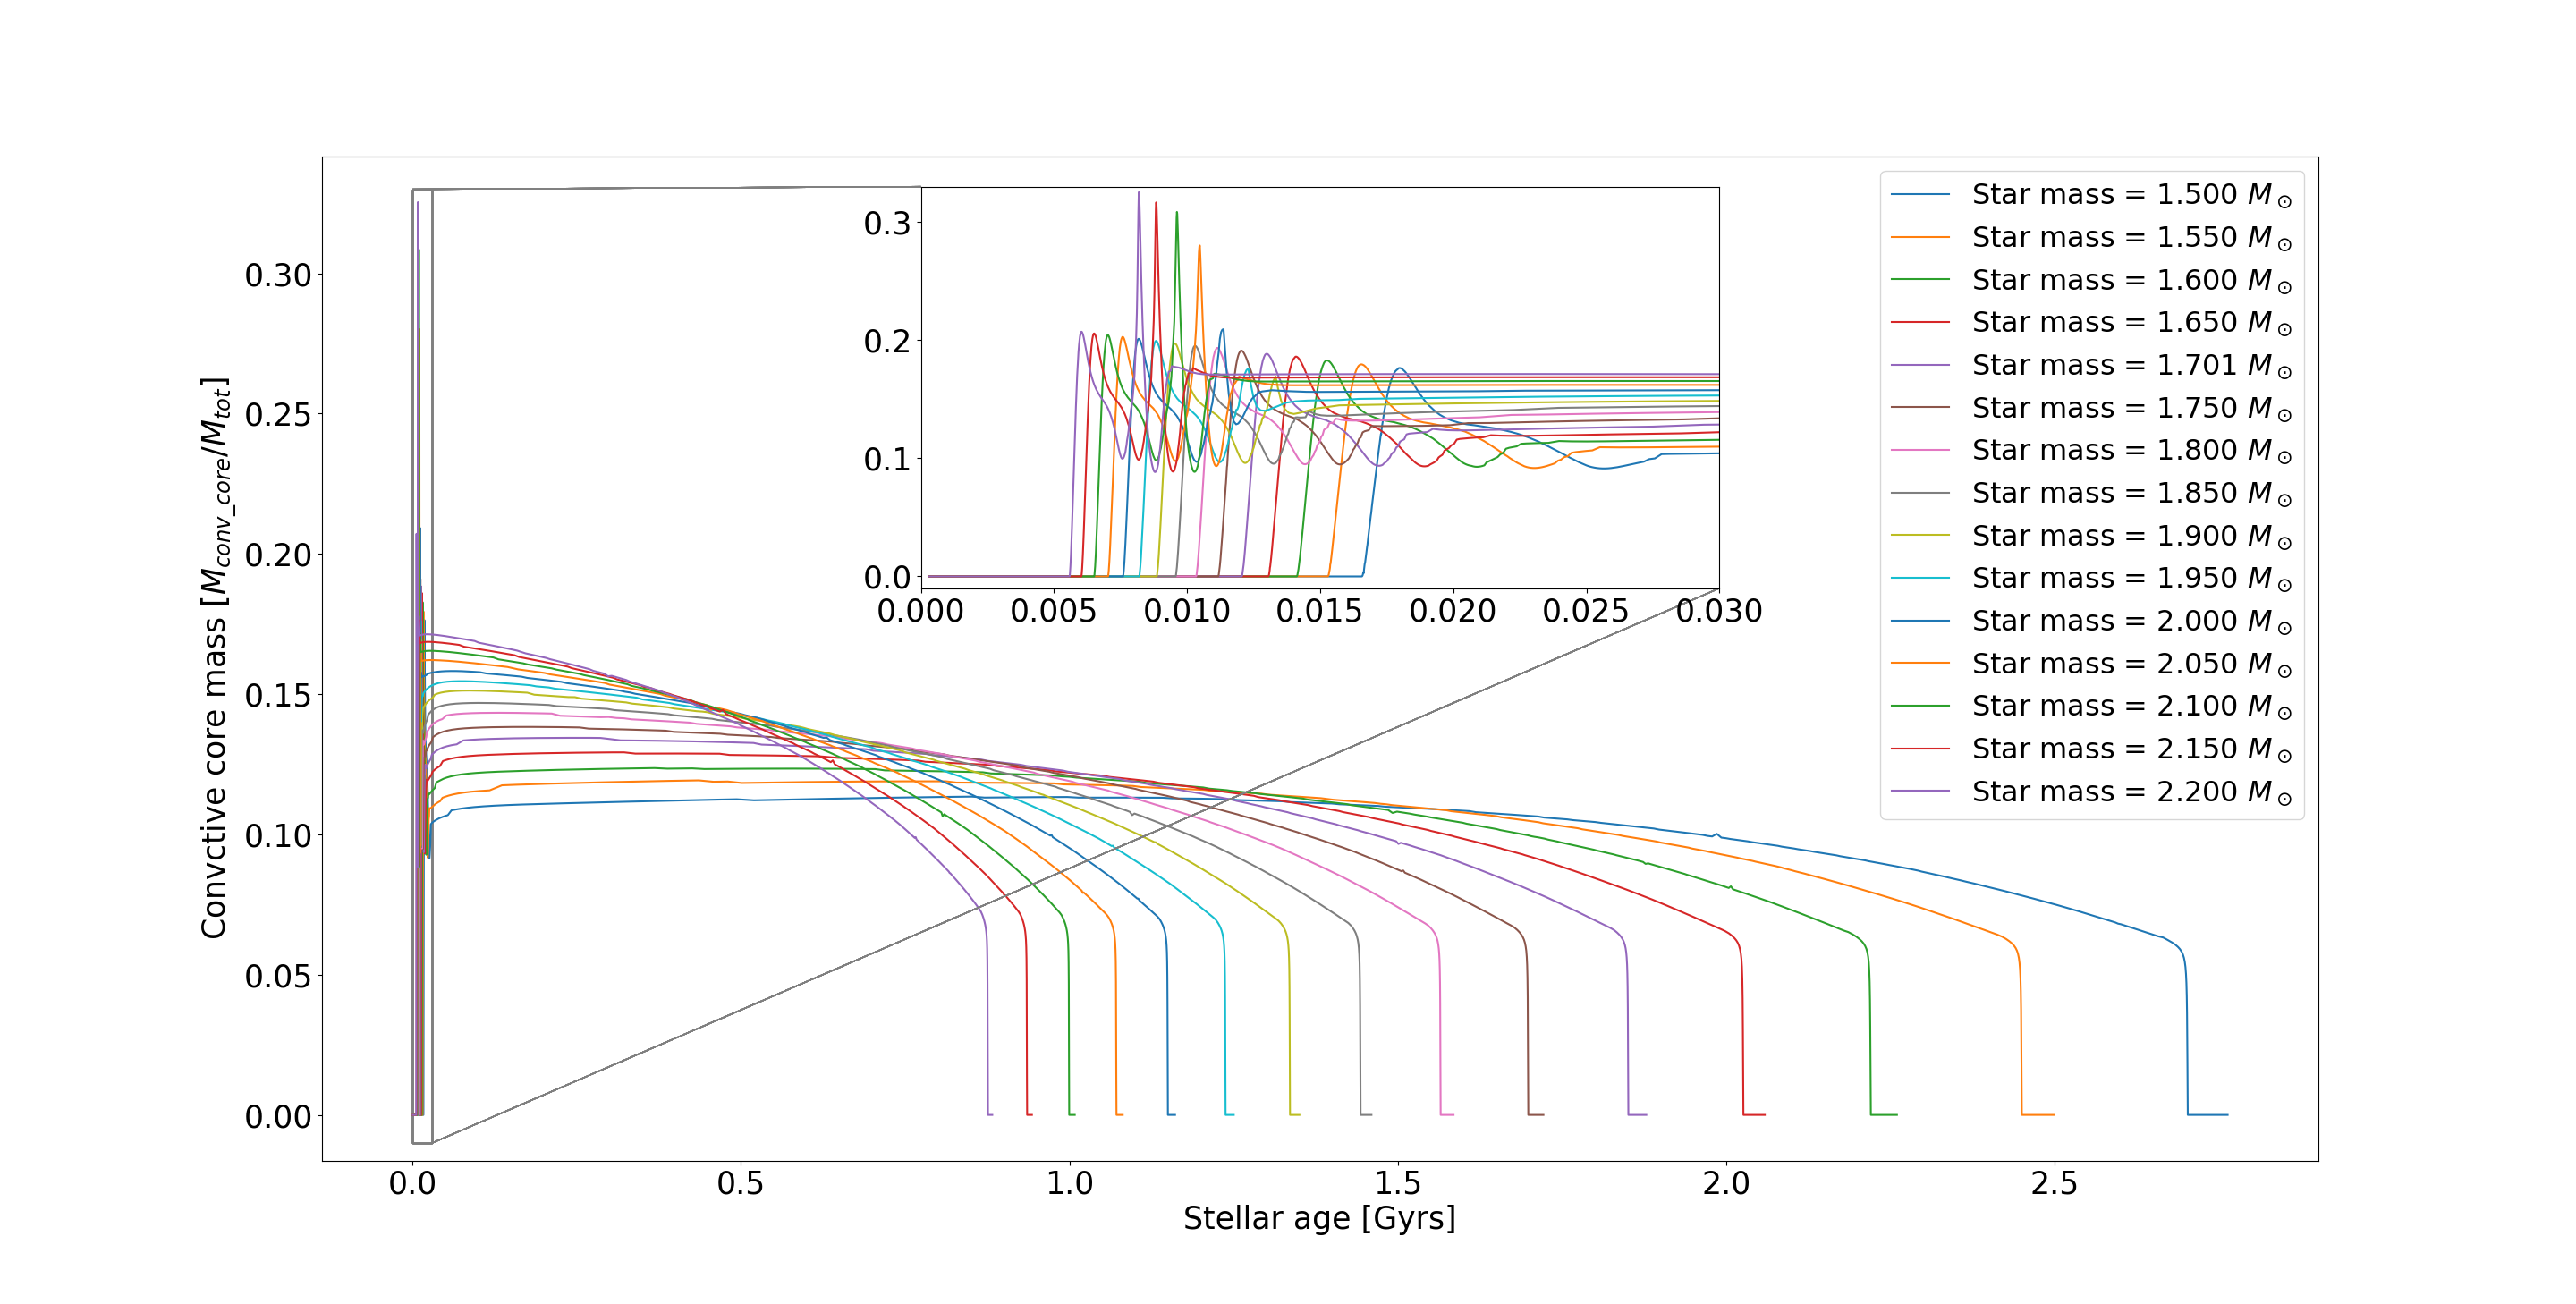
\includegraphics[width=1\textwidth]{conv_cores.png}
    \caption{Numerical results for stars with masses ranging from 1.5\msun to 2.2\msun, X = 0.70, Z = 0.02, $\alpha_{mlt} = 0.5$ and $\alpha_{ov} = 0.3$. The convective core mass ratio is plotted as a function of stellar age. The small window shows a zoom in of the plot at the age where the convective core is established (on the ms)}
    \label{convcore}
\end{figure}

%Regions of convective instability is determined from the instability condition which can be derived from the ideal gas law:

%\begin{equation}
%    \nabla \equiv \frac{d \ln T}{d \ln p} > %\nabla_{ad} + \nabla_{\nu},
%\end{equation}

%\noindent where

%\begin{equation}
 %   \nabla_{ad} = \left(\frac{\partial \ln %T}{\partial \ln p}\right)_{ad},  \nabla_{\mu} = \frac{d \ln \mu }{d \ln p}.
%\end{equation}

%Here, T is the temperature, p is the pressure and $\mu$ is the mean molecular weight.  